\subsection{Proof of Theorem~\ref{structure thm}}
We begin with a proof of Theorem~\ref{structure thm}, and then collect a few preliminary results for later use.

\begin{proof}[Proof of Theorem~\ref{structure thm}]
    Given a permutation $\pi\in \S_{n+1}(p)$, suppose it has the decomposition $\pi=\pi'(n+1)\pi''$ as shown in Fig.~\ref{fig:decomposition of pi(p)}, where the black dot represents the element $n+1$ in $\pi$, while the left square labeled $A^{\sigma}$ refers to the permutation $\pi'$ of
    length $i\,(0\le i\le n)$, and the right square labeled $A^p$ refers to the permutation $\pi''$. The key observation is that $\pi$ is $p$-avoiding if and only if $\pi'$ is $\sigma$-avoiding and $\pi''$ is $p$-avoiding. Consequently, by considering all possible $i$, we have, for $n\ge 0$,
    \begin{equation}\label{eqn-1}
    A_{n+1}^p(t)=t\sum_{i=0}^{n-1}\binom{n}{i}A_i^{\sigma}(t)A_{n-i}^p(t)+A_n^{\sigma}(t).\end{equation}

    \begin{figure}[ht]
        \centering
        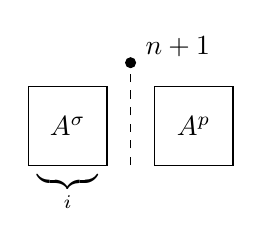
\begin{tikzpicture}
            \draw (-6,5) rectangle (-5,4);
            \fill (-4.7,5.3) circle[radius=2pt];
            \node at (-4.1,5.5) {$n+1$};
            \draw (-4.4,5) rectangle (-3.4,4);
            \draw[dashed] (-4.7,4) -- (-4.7,5.3);
            \node at (-5.5,4.5) {$A^{\sigma}$};
            \node at (-3.9,4.5) {$A^p$};
            \node at (-5.5,3.8) {$\underbrace{\phantom{a+b}}_i$ };
        \end{tikzpicture}
        \caption{A decomposition of $\pi \in \S_{n+1}(p)$}
        \label{fig:decomposition of pi(p)}
    \end{figure}

\noindent
Then, multiplying by $\dfrac{x^n}{n!}$ both sides of (\ref{eqn-1}) and summing over all $n\geq 0$, we obtain
    \begin{align*}
        \sum_{n\ge 0}\frac{A_{n+1}^p(t)x^n}{n!} &= t\sum_{n\ge 0}\sum_{i=0}^{n-1}\frac{A_i^{\sigma}(t)x^i}{i!}\frac{A_{n-i}^p(t)x^{n-i}}{(n-i)!}+\sum_{n\ge 0}A_n^{\sigma}(t)\frac{x^n}{n!} \\
        &= t\sum_{n\ge 0}\sum_{i=0}^{n}\frac{A_i^{\sigma}(t)x^i}{i!}\frac{A_{n-i}^p(t)x^{n-i}}{(n-i)!}-t\sum_{n\ge0}A_n^{\sigma}(t)\frac{x^n}{n!}+\sum_{n\ge 0}A_n^{\sigma}(t)\frac{x^n}{n!} \\
        &= tA^{\sigma}(x,t)A^p(x,t) -tA^{\sigma}(x,t)+A^{\sigma}(x,t).
    \end{align*}

    It follows that $$\sum_{n\ge 0}\frac{A_{n+1}^p(t)x^n}{n!}=\frac{{\partial A^p}}{\partial x}=tA^{\sigma}A^p+(1-t)A^{\sigma}=tA^{\sigma}\left(A^p-1+\frac{1}{t}\right),$$
    where we abbreviate $A^{\sigma}(x,t)$ (resp., $A^p(x,t)$) as $A^{\sigma}$ (resp., $A^p$).
    Setting $\widetilde{A^p}=A^{p}-1+\dfrac{1}{t}$, the initial condition becomes $\widetilde{A^p}(0,t)=\dfrac{1}{t}$ since $A^p(0,t)=1$, and 
    we get $\dfrac{\partial \widetilde{A^p}}{\partial x}=tA^{\sigma}\widetilde{A^p}.$
    Solving this equation with the initial condition, we have 
    $\ln \widetilde{A^p}-\ln \dfrac{1}{t}=t \int_{0}^{x} A^{\sigma}(y,t) \,dy$, and 
    $\widetilde{A^p} = \dfrac{1}{t} e^{t \int_{0}^{x} A^{\sigma}(y,t) \,dy}$.
    Therefore, $A^p = \dfrac{1}{t} e^{t \int_{0}^{x} A^{\sigma}(y,t) \,dy} +1-\dfrac{1}{t}=\dfrac{1}{t} (e^{t \int_{0}^{x} A^{\sigma}(y,t) \,dy}-1) +1$.
\end{proof}

The following result immediately follows from the Structure Theorem, and is useful when we consider the $\des$-Wilf-equivalences for various patterns. It also strengthens Theorem~\ref{thm:eli-kit}.

\begin{corollary}\label{col:structure}
    $\sigma\overset{\des}{\sim}\sigma'$ if and only if $\sigma k\overset{\des}{\sim}\sigma' k$, where $\sigma$ and $\sigma'$ are two consecutive patterns on $\{1,2,\ldots,k-1\}$.
\end{corollary}

Note that the three trivial bijections give rise to obvious Wilf-equivalences such as $123\sim 321$. When we consider $\des$-Wilf-equivalences however, the following result will be handy. For any vincular pattern $\omega$, we abuse the notation and still use $\omega^c$ to denote the vincular pattern whose underlying permutation is the complement of the underlying permutation of $\omega$ with the same set of positions being underlined. For instance, $(\underline{231}4 )^c=\underline{324}1$ and $(\underline{21}4\underline{53})^c=\underline{45}2\underline{13}$. The reverse $\omega^r$ and the reverse-complement $\omega^{cr}=\omega^{rc}$ are understood similarly. So, for example,  $(\underline{231}4 )^r=4\underline{132}$ and $(\underline{21}4\underline{53})^{rc}=\underline{31}2\underline{54}$.

\begin{proposition} \label{omega--omega^rc}
    Let $\omega$ be a vincular pattern, then $\omega \overset{\des}{\sim} \omega^{rc}$, or equivalently $\omega^c \overset{\des}{\sim} \omega^{r}$.
\end{proposition}

\begin{proof}
    It is easily seen that $\des(\pi^{rc})=n-1-\des(\pi^r)=n-1-(n-1-\des(\pi))=\des(\pi)$.
    This indicates that the composition map $\phi_c\circ\phi_r$ preserves the permutation statistic $\des$. Moreover, $\pi \in \S_n(\omega )$ if and only if $\pi^{rc} \in \S_n(\omega^{rc} )$.
    Hence $\omega \overset{\des}{\sim} \omega^{rc}$.
\end{proof}

The following fact will facilitate our derivations of generating functions.

\begin{proposition} \label{omega--omega^c}
    Let $\omega$ be a vincular pattern, then $A^{\omega^c}(x,t)=A^{\omega^r}(x,t)=\dfrac{1}{t} (A^{\omega}(xt,\dfrac{1}{t})-1)+1$.
\end{proposition}

\begin{proof}
    Note that $\des(\pi ^c)=n-1-\des(\pi)$ for $n\ge 1$, and $\pi \in \S_n(\omega) $ if and only if $\pi ^c \in \S_n(\omega^c)$.
    It follows that
    \begin{align*}
        A^{\omega^c}(x,t)&=\sum_{n\ge 0} \sum_{\pi\in \S_n(\omega ^c)} t ^{\des (\pi)}\dfrac{x^n}{n!} \\
        &= \sum_{n\ge 0} \sum_{\pi^c \in \S_n(\omega ^c)} t ^{\des (\pi^c)}\dfrac{x^n}{n!}\\
        &=1+ \sum_{n\ge 1} \sum_{\pi \in \S_n(\omega )} t ^{n-1-\des (\pi)}\dfrac{x^n}{n!}  \\
        &=1+\dfrac{1}{t} \left(A^{\omega}(xt,\dfrac{1}{t})-1\right).
    \end{align*}
   By Proposition~\ref{omega--omega^rc}, $\omega^r \overset{\des}{\sim} \omega^{c}$. Hence, $A^{\omega^c}(x,t) = A^{\omega^r}(x,t)$, completing the proof.
\end{proof}

% Though $\omega$ and $\omega^c$ are not $\des$-Wilf-equivalent, we only need to compute
% the generating function $A^{\omega}(x,t)$ then we naturally know $A^{\omega^c}(x,t)$.


\subsection{Classifications for lengths 2 and 3}

We now provide the complete $\des$-Wilf classification for quasi-consecutive patterns $p = \sigma j$ of length 2 or 3. Using the Structure Theorem, we compute the generating functions $A^p(x, t)$ for all possible choices of $p$, except for $p = \underline{13}2$ and $p = \underline{31}2$. The case of length 2 patterns, $p = \underline{1}2$ and $p = \underline{2}1$, is trivial, as each class contains a unique permutation: $12\cdots n \in \S_n(\underline{2}1)$ and $n(n-1)\cdots 1 \in \S_n(\underline{1}2)$. Their generating functions are straightforward to derive and are included in Table~\ref{tab:2 and 3} for completeness.

% By Proposition~\ref{omega--omega^c}, we only compute the generating function for $\frac{2!}{2}+\frac{3!}{2}=4$ patterns.
% The generating functions about pattern $\sigma k$ of lenth $2$ or $3$ with $\des$ are summarized below.


\begin{table}[h!]
    \setlength{\tabcolsep}{15pt}    %\UTF{8C03}整列\UTF{5BBD}%
    \renewcommand{\arraystretch}{1.2}   %\UTF{8C03}整行距
    \begin{center}
     \begin{tabular}{c|c|c} % <-- Alignments: 1st column left, 2nd middle and 3rd right, with  vertical lines in between
        Pattern $\sigma j$  & $A^{\sigma j}(x,t)$ or $B^{\sigma j}(x,t)$ & Proved in \\ \hline 
        $\underline{1}2$ & $\dfrac{1}{t}(e^{tx}-1)+1$ & N/A  \\ %\hline
        $\underline{2}1$ & $e^{x}$ & N/A  \\ %\hline
        $\underline{12}3$ & $\dfrac{1}{t} (e^{\frac{1}{t}(e^{tx}-1)+x(t-1)}-1)+1$ & Theorem~\ref{thm:12-3 and 21-3} \\ %\hline
        $\underline{32}1$ & $e^{t(e^{x}-1)+x(1-t)}$ & Corollary~\ref{cor:32-1 and 23-1} \\ %\hline
        $\underline{21}3$ & $\dfrac{1}{t} (e^{t(e^x-1)}-1)+1$ & Theorem~\ref{thm:12-3 and 21-3} \\ %\hline
        $\underline{23}1$ & $e^{\frac{1}{t}(e^{xt}-1)}$ &  Corollary~\ref{cor:32-1 and 23-1} \\ %\hline
        $\underline{13}2$, $\underline{31}2$ & $\dfrac{1+x(t-1)-\sqrt{1-2x(t+1)+x^2(t-1)^2}}{2tx}$ &  Proposition~\ref{13-2}
        \end{tabular}
  \end{center}
  \caption{The $\des$-Wilf classifications of pattern $\sigma j$ whose length is $2$ or $3$}
  \label{tab:2 and 3}
\end{table}

% \begin{proposition} \label{1-2}
%     $A^{\underline{1}2}(x,t)=\dfrac{1}{t}(e^{tx}-1)+1.$
% \end{proposition}

% \begin{proof}
%     By Theorem~\ref{structure thm}, we fistly compute $A^{\underline{1}}(x,t)$.
%     Actually, $A^{\underline{1}}(x,t)=A^{1}(x,t)$, and it records the descent of the empty permutation.
%     Hence, $A^{1}(x,t)=A_0^{1}(t)=1$. Putting it into the equation in Theorem~\ref{structure thm} gets $A^{\underline{1}2}(x,t)$.
% \end{proof}

% Using Proposition~\ref{omega--omega^c}, we have $A^{\underline{2}1}(x,t)$, see follows.

% \begin{corollary} \label{2-1}
%     $A^{\underline{2}1}(x,t)=e^{x}.$
% \end{corollary}

Next, we compute the generating functions for patterns of length 3. Among all six patterns, only half of the derivations (one from each complementary pair) are necessary, thanks to Proposition~\ref{omega--omega^c}.

\begin{theorem} \label{thm:12-3 and 21-3}
    We have
    \begin{align*}
    A^{\underline{12}3}(x,t) &= \dfrac{1}{t} (e^{\frac{1}{t}(e^{tx}-1)+x(t-1)}-1)+1,\\
    A^{\underline{21}3}(x,t) &= \dfrac{1}{t} (e^{t(e^x-1)}-1)+1.
    \end{align*}
\end{theorem}

\begin{proof}
    We first compute $A^{\underline{12}}(x,t)$. Clearly, $\S_n(\underline{12})=\S_n(12)=\S_n(\underline{1}2)=\{n(n-1)\cdots 1\}$. Hence $A^{\underline{12}}(x,t)=A^{\underline{1}2}(x,t)=\dfrac{1}{t}(e^{tx}-1)+1$.
    By Theorem~\ref{structure thm}, we have 
    $\displaystyle{A^{\underline{12}3}(x,t)=\frac{1}{t} (e^{t \int_{0}^{x} A^{\underline{12}}(y,t) \,dy}-1) +1 }$, while 
    \begin{align*}
        \int_{0}^{x} A^{\underline{12}}(y,t) \,dy &=\int_{0}^{x} \left(\frac{1}{t}(e^{ty}-1)+1\right)\,dy \\
        &= \left. \left(\frac{1}{t}(\frac{1}{t} e^{ty}-y)+y\right) \right|_{0}^{x} \\
%        &=\frac{1}{t^2} e^{tx}-\frac{x}{t}+x-\frac{1}{t^2} \\
        &= \frac{1}{t^2}(e^{tx}-1)+\frac{x}{t}(t-1).
    \end{align*}
    We thus obtain $\displaystyle{A^{\underline{12}3}(x,t)=\frac{1}{t} (e^{\frac{1}{t}(e^{tx}-1)+x(t-1)}-1)+1}$, as desired. The derivation of $A^{\underline{21}3}(x,t)$ is similar and is omitted.
\end{proof}

Applying Proposition~\ref{omega--omega^c}, we immediately get the generating functions for two complementary patterns through simple calculation.

\begin{corollary} \label{cor:32-1 and 23-1}
    We have
    \begin{align*}
    A^{\underline{32}1}(x,t) &= e^{t(e^{x}-1)+x(1-t)},\\
    A^{\underline{23}1}(x,t) &= e^{\frac{1}{t}(e^{xt}-1)}.
    \end{align*}
\end{corollary}

\begin{remark}
It is worth noting that when we plug in $t=1$ for each of the four generating functions contained in Theorem~\ref{thm:12-3 and 21-3} and Corollary~\ref{cor:32-1 and 23-1}, they all reduce to $e^{e^x-1}$, which is the well-known exponential generating function for the Bell numbers $\{B_n\}_{n\ge 0}=\{1,1,2,5,15,52,203,877,\ldots\}$; see \href{https://oeis.org/A000110}{\tt{oeis:A000110}}. This enumerative fact was first observed by Claesson~\cite[Prop.~2 and 3]{cla01}. In fact, Claesson constructed two bijections between pattern avoiding permutations and set partitions to establish that
\begin{align}\label{id:perm-setpar}
|\S_n(1\underline{23})|=|\S_n(1\underline{32})|=B_n.
\end{align}
\end{remark}

Taking into consideration the effect of these bijections on the descent numbers of pattern avoiding permutations, we are naturally led to the following refinement of \eqref{id:perm-setpar}. Let $\Par_n$ be the collection of all set partitions of $[n]$. Given a set partition $\Pi\in\Par_n$, we denote by $\blk(\Pi)$ and $\sing(\Pi)$ the number of blocks and the number of singletons (i.e., $1$-blocks) of $\Pi$, respectively. For example, the set partition $\Pi=135/2/4689/7\in\Par_9$ satisfies $\blk(\Pi)=4$ and $\sing(\Pi)=2$.

\begin{corollary}
We have the following alternative interpretations of the generating functions:
\begin{align}
\label{id:gf321 in setpar}
A^{\underline{32}1}(x,t) &= \sum_{n\ge 0}\sum_{\Pi\in\Par_n}t^{\blk(\Pi)-\sing(\Pi)}\frac{x^n}{n!},\\
A^{\underline{21}3}(x,t) &= \sum_{n\ge 0}\sum_{\Pi\in\Par_n}t^{\blk(\Pi)-1}\frac{x^n}{n!}.
\label{id:gf213 in setpar}
\end{align}
\end{corollary}

\begin{proof}
We begin with the proof of \eqref{id:gf321 in setpar}. In view of the original definition of $A^{\underline{32}1}(x,t)$, it suffices to show that the statistic ``$\des$'' over $\S_n(\underline{32}1)$ is equidistributed with ``$\blk -\sing$'' over $\Par_n$. Combining the bijection constructed in Claesson's second proof of \cite[Prop.\ 2]{cla01} with the reversal map $\phi_r$, we get a bijection, say $\varphi$, from $\Par_n$ to $\S_n(\underline{32}1)$ that can be explicitly described as follows. Given a partition $\Pi\in\Par_n$, we say it is expressed in the \textit{standard representation} if the following conditions are enforced:
\begin{enumerate}[label=(\roman*)]
    \item Each block ends with its smallest element, and all remaining elements are written in increasing order.
    \item The blocks are written in increasing order of their smallest element with slashes separating the blocks.
\end{enumerate}
The standard representation for the previous set partition $\Pi$ is seen to be $351/2/6894/7$. Next, we simply remove all the slashes to get its image permutation $\pi=\varphi(\Pi)$. Clearly, the descents of $\pi$ are precisely between the penultimate and the ending elements within each non-singleton block of $\Pi$ (in its standard representation). This not only implies that $\pi$ is $\underline{32}1$-avoiding, but also reveals the relation $\des(\pi)=\blk(\Pi)-\sing(\Pi)$. To see that $\varphi$ is indeed invertible, note that one can recover the preimage $\varphi^{-1}(\pi)$ in its standard representation by inserting a slash after every right-to-left minimum of $\pi$. 

The proof of \eqref{id:gf213 in setpar} is in the same vein but with the following conditions on \textit{another standard representation} of set partitions:
\begin{enumerate}[label=(\roman*)]
    \item The elements in each block are written in increasing order.
    \item The blocks are written in decreasing order of their last (also largest) element with slashes separating the blocks. \qedhere
\end{enumerate}
\end{proof}

% The generating function of $\S_n(\underline{12}3)$ is
% $A^{\underline{12}3}(x,1)=e^{(e^{x}-1)}=\sum_{\pi \in \S_n(\underline{12}3)} B_n \dfrac{x^n}{n!}$, where $B_n$ is the $n$-th Bell number.
% Claesson~\cite{cla01} has proved that the set partitions of $[n]:=\{1,2,\cdots,n\}$ is one-to-one corresponding to the permutations 
% of length $n$ avoiding $1\underline{23}$.
% Given a permutation $\pi \in \S_n(1\underline{23})$, let $\varphi(\pi)$ be the corresponding set partition of $[n]$.
% For example, the permutation $\pi =847296153$ corresponds to the set partition $\varphi(\pi)= \{(1,3,5),(2,6,9),(4,7),(8) \}$.
% We also have $\des(\pi)=n-1-\mathrm{cyc}(\varphi(\pi))+\mathrm{sing}(\varphi(\pi))$ by the second proof of Proposition~2 in \cite{cla01},
% where $\mathrm{cyc}(\varphi(\pi))$ is the number of blocks in $\varphi(\pi)$ and $\mathrm{sing}(\varphi(\pi))$ is the number of singleton in $\varphi(\pi)$.

% By Theorem~\ref{omega--omega^rc}, the bijection $\phi_c\circ\phi_r\circ\varphi$ indicates the set partitions of $[n]$ is one-to-one corresponding to the permutations 
% of length $n$ avoiding $\underline{12}3$ and $\des(\pi)=\des(\pi^{rc})=n-1-\mathrm{cyc}(\varphi(\pi^{rc}))+\mathrm{sing}(\varphi(\pi^{rc}))$ for $\pi \in \S_n(\underline{12}3)$.

% Similarly, $\des(\pi)=n-1-\des(\pi^{r})=n-1-(n-1-\mathrm{cyc}(\varphi(\pi^{r}))+\mathrm{sing}(\varphi(\pi^{r})))=\mathrm{cyc}(\varphi(\pi^{r}))-\mathrm{sing}(\varphi(\pi^{r}))$ for $\pi \in \S_n(\underline{32}1)$.


% \begin{proof}
%     Firstly, we compute $A^{\underline{21}}(x,t)$. 
%     Similarly, we have $\S_n(\underline{21})=\S_n(21)=\S_n(\underline{2}1)$ for all $n$.
%     Hence $A^{\underline{21}}(x,t)=A^{\underline{2}1}(x,t)=e^x.$
%     By Theorem~\ref{structure thm}, we have
%     $$A^{\underline{21}3}(x,t) =\frac{1}{t} (e^{t \int_{0}^{x} A^{\underline{21}}(y,t) \,dy}-1) +1 
%        = \frac{1}{t} (e^{t \int_{0}^{x} e^y \,dy}-1) +1 =\frac{1}{t} (e^{t (e^x-1)}-1) +1,$$
%     finish the computation.
% \end{proof}



% The generating function of $\S_n(\underline{21}3)$ is
% $A^{\underline{21}3}(x,1)=e^{(e^{x}-1)}=\sum_{\pi \in \S_n(\underline{12}3)} B_n \dfrac{x^n}{n!}$.
% Claesson~\cite{cla01} also proved that the set partitions of $[n]$ is one-to-one corresponding to the permutations 
% of length $n$ avoiding $1\underline{32}$. 
% Given a permutation $\pi \in \S_n(1\underline{32})$, let $\psi (\pi)$ be the corresponding set partition of $[n]$.
% For example, the permutation $\pi =847269135$ corresponds to the set partition $\psi(\pi)= \{(1,3,5),(2,6,9),(4,7),(8) \}$.
% The correspondence $\psi$ satisfies $\des(\pi)=\mathrm{cyc}(\psi(\pi))-1$.
% Similarly, $\des(\pi)=\des(\pi^{rc})=\mathrm{cyc}(\psi(\pi^{rc}))-1$ for $\pi \in \S_n(\underline{21}3)$.

% Moreover, $\des(\pi)$ for $\pi \in \S_n(\underline{21}3)$ has following property.

% \begin{theorem}
%     Let $\pi \in \S_n(\underline{21}3)$. Then 
%     $\des(\pi)=\mathrm{rlmax}(\pi)-1$, where $\mathrm{rlmax}(\pi)$ is the number of the right-to-left maximum of $\pi$.
% \end{theorem}

% \begin{proof}
%     We claim that if $\pi_i>\pi_{i+1}$ for some $1\le i \le n-1$, then $\pi_i$ is a right-to-left maximum of $\pi$.
%     Note if $i=n-1$, $\pi_i>\pi_{i+1}$ makes $\pi_i$ be a right-to-left maximum of $\pi$.
%     We prove this claim by contradiction.
%     Assume that $\pi_i>\pi_{i+1}$ for some $1\le i < n-1$ and $\pi_i$ is not a right-to-left maximum of $\pi$.
%     The second condition means there exist elements $\pi_k$ for $i+1<k\le n$ such that $\pi_i<\pi_k$.
%     Then $\pi_i\pi_{i+1}\pi_k$ forms a pattern $\underline{21}3$, it contradicts $\pi \in \S_n(\underline{21}3)$.
%     Therefore, the claim holds.
%     Notice $\pi_n$ must be a right-to-left maximum of $\pi$. So $\mathrm{rlmax}(\pi)-1 \ge \des(\pi)$.

%     On the other hand, the right-to-left maximum of $\pi$ makes the descent number increasing $1$ except the first right-to-left maximum $\pi_n$. 
%     Thus $\mathrm{rlmax}(\pi)-1 \le \des(\pi)$. 

%     \begin{figure}[ht]
%         \centering
%         \begin{tikzpicture}
%             \draw (-6,6) rectangle (-4,4);
%             \draw[dashed] (-6,4) -- (-4,6);
%             \fill (-3.7,6.3) circle[radius=2pt];
%             \node at (-3.5,6.4) {$n$};
%             \draw (-3.4,6) rectangle (-2.9,5.5);
%             \draw[dashed] (-3.4,5.5) -- (-2.9,6);
%             \fill (-2.9,6) circle[radius=2pt];
%             \draw (-2.9,5.5) rectangle (-2.4,5);
%             \draw[dashed] (-2.9,5) -- (-2.4,5.5);
%             \fill (-2.4,5.5) circle[radius=2pt];
%             \draw (-2.4,5) rectangle (-1.9,4.5);
%             \draw[dashed] (-2.4,4.5) -- (-1.9,5);
%             \fill (-1.9,5) circle[radius=2pt];
%             \draw (-1.9,4.5) rectangle (-1.4,4);
%             \draw[dashed] (-1.9,4) -- (-1.4,4.5);
%             \fill (-1.4,4.5) circle[radius=2pt];
%         \end{tikzpicture}
%         \caption{Decomposition of $\pi\in \S_n(\underline{21}3)$}
%         \label{fig:decomposition of pi(21-3)}
%     \end{figure}
%     To sum up, we get $\des(\pi)=\mathrm{rlmax}(\pi)-1$.
%     We draw a Figure to illustrate this result. In Figure~\ref{fig:decomposition of pi(21-3)}, the
%     black dot represents a right-to-left maximum of $\pi$, the square with diagonal dotted line means the elements
%     in square are increasing and they are smaller than the nearest black dot on the right.
% \end{proof}


% Similarly, $\des(\pi)=n-1-\des(\pi^{r})=n-1-(\mathrm{cyc}(\psi(\pi^{r}))-1)=n-\mathrm{cyc}(\psi(\pi^{r}))$ for $\pi \in \S_n(\underline{23}1)$.

For the remaining pair of patterns $\underline{13}2$ and $\underline{31}2 = (\underline{13}2)^c$, the Structure Theorem is inapplicable, as neither of them ends with the largest element. Moreover, it was already noted in \cite[Lem.\ 2]{cla01} (see also \cite[Lem.\ 2.8]{FTHZ19}) that \begin{align*} \S_n(\underline{13}2) = \S_n(132), \quad \S_n(\underline{31}2) = \S_n(312), \ \S_n(2\underline{13}) = \S_n(213), \quad \S_n(2\underline{31}) = \S_n(231). \end{align*} Hence, all of them are enumerated by the {\em Catalan numbers} $C_n = \frac{1}{n+1}\binom{2n}{n}$. Based on these observations, we instead consider the ordinary generating function $B^{\omega}(x,t) = \sum_{n \geq 0} \sum_{\pi \in \S_n(\omega)} t^{\des(\pi)} x^n$ for the last two patterns. The relation in Proposition~\ref{omega--omega^c} still holds, with $A^{\omega}(x,t)$ replaced by $B^{\omega}(x,t)$.

\begin{proposition} \label{13-2}
    We have
    \begin{align*}
    B^{\underline{13}2}(x,t) = B^{\underline{31}2}(x,t)= \dfrac{1+x(t-1)-\sqrt{1-2x(t+1)+x^2(t-1)^2}}{2tx}.
    \end{align*}
\end{proposition}

\begin{proof}
By Proposition~\ref{omega--omega^rc}, we know that $\underline{31}2 \overset{\des}{\sim} 2\underline{31}$. Now the descent distribution over $\S_n(2\underline{31})=\S_n(231)$ generates the {\em Narayana polynomial} $N_n(t):=\sum_{0\le k\le n-1}N_{n,k}t^k$, where
$$N_{n,k}:=|\{\pi\in \S_n(231):\des(\pi)=k\}|=\frac{1}{k+1}\binom{n}{k}\binom{n-1}{k}$$
is the \textit{Narayana number}. The ordinary generating function of Narayana polynomials $N_n(t)$ is known to be (for instance, see \cite[Sect.~2.3]{pet15})
$$B^{231}(x,t)=\dfrac{1+x(t-1)-\sqrt{1-2x(t+1)+x^2(t-1)^2}}{2tx},$$
which gives the desired expression for $B^{\underline{31}2}(x,t)$. To derive the same formula for $B^{\underline{13}2}(x,t)$, we simply apply Proposition~\ref{omega--omega^c} and perform the derivations. Alternatively, it suffices to note the palindromicity of Narayana numbers (i.e., $N_{n,k}=N_{n,n-1-k}$) and the relation $\des(\pi^r)=n-1-\des(\pi)$ that holds for all $\pi\in\S_n$.
\end{proof}


% \underline{13}2 和 \underline{31}2 之\UTF{95F4}的双射???


